\documentclass[twoside]{article}
\usepackage{format/aistats2e}
\usepackage{amssymb,amsmath,amsthm}
\usepackage{graphicx}
\usepackage{preamble}
\usepackage{natbib}
\usepackage{hyperref}
\usepackage{color}
\definecolor{mydarkblue}{rgb}{0,0.08,0.45}
\hypersetup{ %
    pdftitle={},
    pdfauthor={},
    pdfsubject={},
    pdfkeywords={},
    pdfborder=0 0 0,
    pdfpagemode=UseNone,
    colorlinks=true,
    linkcolor=mydarkblue,
    citecolor=mydarkblue,
    filecolor=mydarkblue,
    urlcolor=mydarkblue,
    pdfview=FitH}
    
    
% If your paper is accepted, change the options for the package
% aistats2e as follows:
%
%\usepackage[accepted]{aistats2e}
%
% This option will print headings for the title of your paper and
% headings for the authors names, plus a copyright note at the end of
% the first column of the first page.


\begin{document}

% If your paper is accepted and the title of your paper is very long,
% the style will print as headings an error message. Use the following
% command to supply a shorter title of your paper so that it can be
% used as headings.
%
%\runningtitle{I use this title instead because the last one was very long}

% If your paper is accepted and the number of authors is large, the
% style will print as headings an error message. Use the following
% command to supply a shorter version of the authors names so that
% they can be used as headings (for example, use only the surnames)
%
%\runningauthor{Surname 1, Surname 2, Surname 3, ...., Surname n}

\twocolumn[

\aistatstitle{Structure Search in Gaussian Process Models}

\aistatsauthor{ Anonymous Author 1 \And Anonymous Author 2 \And Anonymous Author 3 }

\aistatsaddress{ Unknown Institution 1 \And Unknown Institution 2 \And Unknown Institution 3 } ]

\begin{abstract}
Gaussian process (GP) models are used widely and successfully.  However, their effictiveness depends critically on choosing an appropriate family of kernels.  This aspect of GP modeling has been sorely underdeveloped.  In this paper, we introduce a procedure for automatically and efficiently searching through a large space of GP models.
\end{abstract}

\section{INTRODUCTION}

Expand on what was said in the abstract.  Cite \cite{rasmussen38gaussian}

\section{RELATED WORK}


Model search \cite{grosse2012exploiting}

Additive Gaussian Processes \cite{duvenaud2011additive11}

Genetic Programming work

Equation Learning

Hyperkernels

\begin{figure}
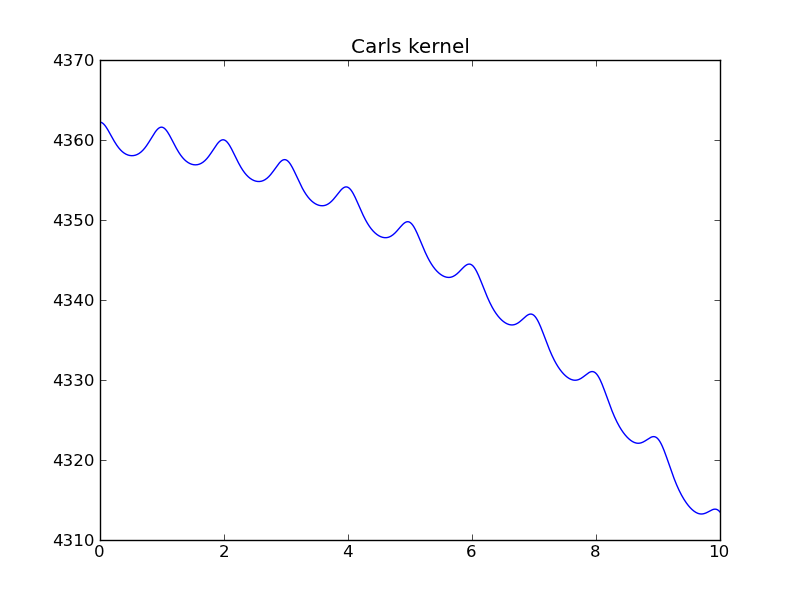
\includegraphics[width=\columnwidth]{../figures/carls_kernel}
\caption{Carl's kernel function on the Mauna dataset.}
\end{figure}

\begin{figure}
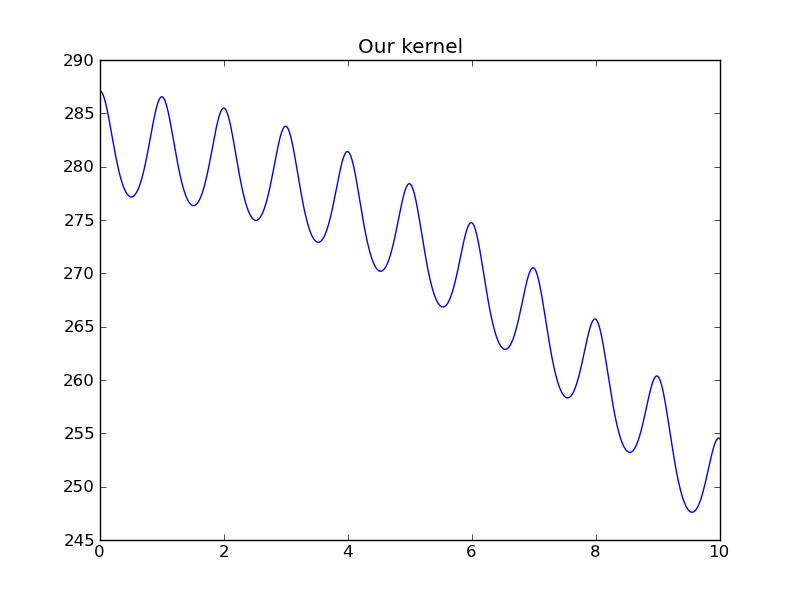
\includegraphics[width=\columnwidth]{../figures/our_kernel}
\caption{Our best kernel function on the Mauna dataset.}
\end{figure}

\begin{figure}[h]
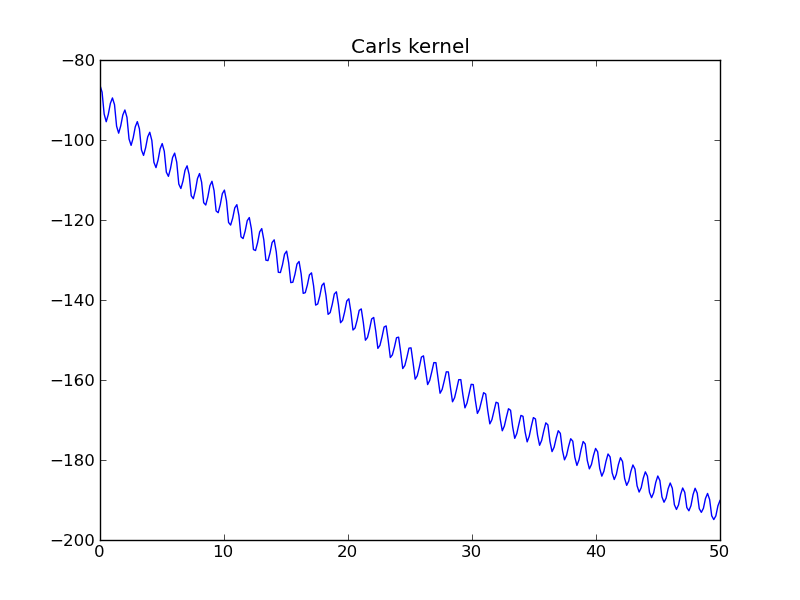
\includegraphics[width=\columnwidth]{../figures/carls_kernel_draw1}
\caption{A draw from Carl's kernel.}
\end{figure}

\begin{figure}[h]
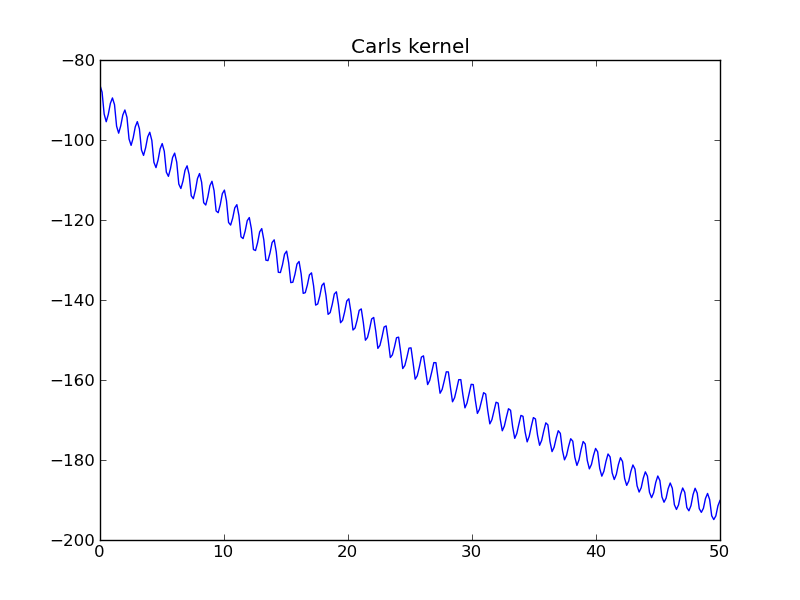
\includegraphics[width=\columnwidth]{../figures/carls_kernel_draw1}
\caption{Another draw from Carl's kernel.}
\end{figure}

\begin{figure}[h]
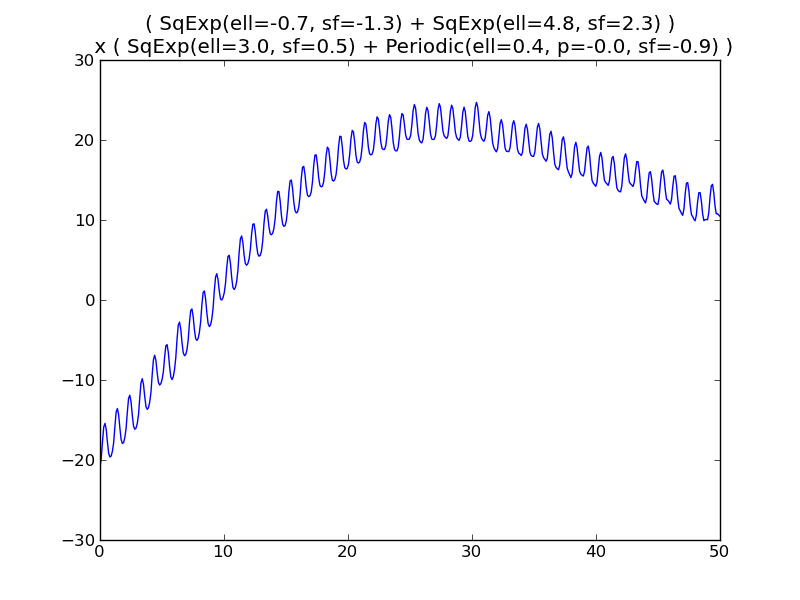
\includegraphics[width=\columnwidth]{../figures/mauna_prior_draw_best_cov_v3}
\caption{Another draw from our kernel.}
\end{figure}

\begin{figure}[h]
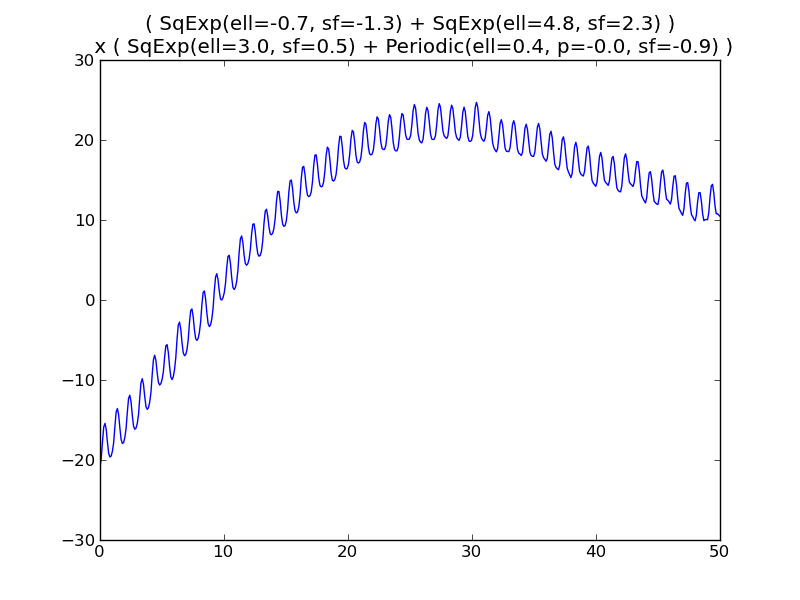
\includegraphics[width=\columnwidth]{../figures/mauna_prior_draw_best_cov_v3}
\caption{Another draw from our kernel.}
\end{figure}


\subsubsection*{Acknowledgements}


\bibliographystyle{format/icml2013}
\bibliography{gpss}

\end{document}
